\begin{flushright} {\tiny {\color{gray} fdm\_adv1D.tex}} \end{flushright}

%TODO to improve notes:
%use http://farside.ph.utexas.edu/teaching/329/lectures/node91.html
%


The 1D advection equation is:
\begin{equation}
\rho C_p \left( \frac{\partial T}{\partial t}  
+ u \frac{\partial T}{\partial x} \right)=0 
\end{equation}
or simply
\begin{equation}
\frac{\partial T}{\partial t} + u \frac{\partial T}{\partial x}=0 
\end{equation}
We have seen how to deal with the time derivative (explicit, implicit) 
and with the first order space derivative (forward, backward or central).
Let us consider the FTCS scheme (Forward in Time, Central in Space).
\[
\frac{T_{\color{teal}i}^{n+1}-T^n_{\color{teal}i}}{\delta t} 
+ u_i \frac{T^n_{\color{teal}i+1} - T^n_{{\color{teal}i-1}}}{2h} =0 
\]
Note that although the velocity $u$ is prescribed, it can vary in space, hence
the subscript $i$. 

There is however a major problem: 
the FTCS method is in this case {\bf unconditionally} {\bf un}stable, i.e., it blows up for any $\delta t$.
The instability is related to the fact that this scheme produces negative diffusion, 
which is numerically unstable.

We will now look at to methods which alleviate this problem: the Lax method and the Streamline Upwind method.

The {\color{olive} Lax method} consists of replacing the $T_{\color{teal}i}^n$ 
in the time derivative term with $(T_{{\color{teal}i+1}}^n + T_{{\color{teal}i-1}}^n)/2$. 
The resulting equation is
\[
\frac{T_{\color{teal}i}^{n+1}-  (T_{{\color{teal}i+1}}^n + T_{{\color{teal}i-1}}^n)/2 }{\delta t} 
= - u_i \frac{T^n_{{\color{teal}i+1}}-T^n_{{\color{teal}i-1}}}{2 h}
\]
or, 
\[
T_{\color{teal}i}^{n+1} = \frac{1}{2} (T_{{\color{teal}i+1}}^n + T_{{\color{teal}i-1}}^n)  
- \frac{u_i \delta t}{h}  \frac{1}{2} (T^n_{{\color{teal}i+1}}-T^n_{{\color{teal}i-1}})
\]



In the {\color{olive}Streamline upwind} method the spatial finite difference scheme 
depends on the sign of the velocity:
\[
\frac{T_{\color{teal}i}^{n+1}-  (T_{{\color{teal}i+1}}^n + T_{{\color{teal}i-1}}^n)/2   }{\delta t} =
\left\{
\begin{array}{l}
 - u_i \frac{T^n_{{\color{teal}i}}-T^n_{{\color{teal}i-1}}}{h_x}  \quad\quad  {\rm if} \quad u_i<0\\ \\
 - u_i \frac{T^n_{{\color{teal}i+1}}-T^n_{{\color{teal}i}}}{h_x}  \quad\quad  {\rm if} \quad u_i>0
\end{array}
\right.
\]
In fact, we have replaced central with forward or backward derivatives, depending on the flow direction. 


Finally, The Crank-Nicolson implicit scheme for solving the diffusion equation 
can be adapted to solve the advection equation:
\[
T_{\color{teal}i}^{n+1} + \frac{u \delta t}{4h} (T_{{\color{teal}i+1}}^{n+1}-T_{{\color{teal}i-1}}^{n+1}) 
= T_{\color{teal}i}^n - \frac{u \delta t}{4h} (T_{{\color{teal}i+1}}^{n}-T_{{\color{teal}i-1}}^{n}) 
\]
TODO: write about how we obtain this.


%-/-/-/-/-/-/-/-/-/-/-/-/-/-/-/-/-/-/-/
\begin{center}
\begin{minipage}[t]{0.77\textwidth}
\par\noindent\rule{\textwidth}{0.4pt}

\begin{center}

\includegraphics[width=0.8cm]{images/garftr} \\
{\color{orange}Exercise FDM-6}
\end{center}

Let us consider the domain $[0,1]$. The temperature field at $t=0$ is 
given by $T=1$ for $x<0.25$ and $T=0$ otherwise. The prescribed 
velocity is $u=1$ and we set $nnx=51$.
Boundary conditions are $T=1$ at $x=0$ and $T=0$ at $x=1$.

\begin{center}

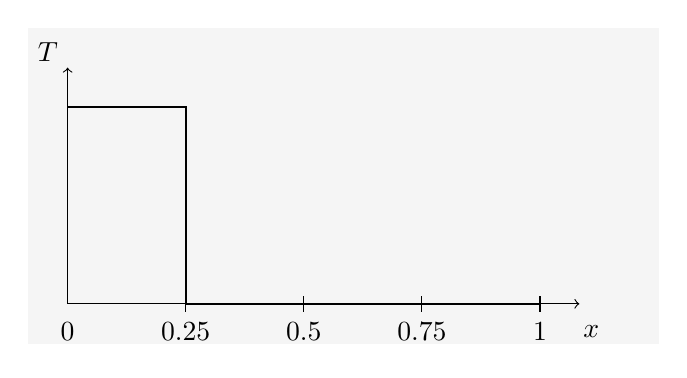
\begin{tikzpicture}
\draw[fill=gray!8,gray!8](0,0) rectangle (8,4);
%\draw[step=0.5cm,gray,very thin] (0,0) grid (8,4); %background grid

\draw[->] (0.5,0.5) -- (7,0.5) ; 
\node[] at (0.5,0.15) {$0$};

\node[] at (2,0.15) {$0.25$};
\node[] at (3.5,0.15) {$0.5$};
\node[] at (5,0.15) {$0.75$};
\node[] at (6.5,0.15) {$1$};
\draw[->] (0.5,0.5) -- (0.5,3.5) ; 
\node[] at (0.25,3.7) {$T$};


\draw[-] (2,0.4) -- (2,0.6) ; 
\draw[-] (3.5,0.4) -- (3.5,0.6) ; 
\draw[-] (5,0.4) -- (5,0.6) ; 
\draw[-] (6.5,0.4) -- (6.5,0.6) ; 


%\draw[-] (2,1) -- (1.75,0.75) ; 
%\draw[-] (2.5,1) -- (2.25,0.75) ; 
%\draw[-] (3,1) -- (2.75,0.75) ; 
%\draw[-] (3.5,1) -- (3.25,0.75) ; 
%\draw[-] (4,1) -- (3.75,0.75) ; 
%\draw[-] (4.5,1) -- (4.25,0.75) ; 

%---------------------------------

%\draw[thick,->] (7,1) -- (7,5) ; 
%\node[] at (6.6,4) {$L_y$};
%\node[] at (6.6,1) {$0$};
%\draw[-] (6.85,1) -- (7.15,1) ; 
%\draw[-] (6.85,4) -- (7.15,4) ; 
%\node[] at (7.6,4) {$p=0$};
%\node[] at (6.6,5) {$y$};

%---------------------------------

\draw[thick] (0.5,3) -- (2,3) -- (2,0.5) -- (6.5,0.5) ; 
\node[] at (7.15,0.15) {$x$};


\end{tikzpicture}



\end{center}

Program the above FTCS method. Run the model for 250 time steps with $\delta t=0.002$. 
Program the Lax method by modifying the previous code.\\
Bonus: Program the upwind method and/or the Crank-Nicolson method. 

\par\noindent\rule{\textwidth}{0.4pt}
\end{minipage}
\end{center}
%-/-/-/-/-/-/-/-/-/-/-/-/-/-/-/-/-/-/



